% This is samplepaper.tex, a sample chapter demonstrating the
% LLNCS macro package for Springer Computer Science proceedings;
% Version 2.20 of 2017/10/04
%
\documentclass[runningheads]{llncs}
%
\usepackage{graphicx}

\begin{document}
%
\title{Your Project Title}

\author{Group Name: First Author \and
Second Author \and
Third Author}

\institute{Service Computing Department, IAAS, University of Stuttgart
\email{firstname.lastname@uni-stuttgart.de}}
%
\maketitle              % typeset the header of the contribution
%
\begin{abstract}
The abstract should briefly summarize the contents of the report in
150--250 words.

\keywords{First keyword  \and Second keyword \and Another keyword.}
\end{abstract}
%
%
%
\section{Introduction}
Please note that the first paragraph of a section or subsection is
not indented. The first paragraph that follows a table, figure,
equation etc. does not need an indent, either.

Subsequent paragraphs, however, are indented.

Table~\ref{tab1} an example of a table.

\begin{table}
\caption{Table captions should be placed above the
tables.}\label{tab1}
\begin{tabular}{|l|l|}
\hline
Item & Deadline \\
\hline
I1 & D1 \\
I2 & D2 \\
I3 & D3 \\
I4 & D4 \\
I5 & D5 \\
\hline
\end{tabular}
\end{table}

Fig.~\ref{fig1} gives an example of a figure.

\begin{figure}
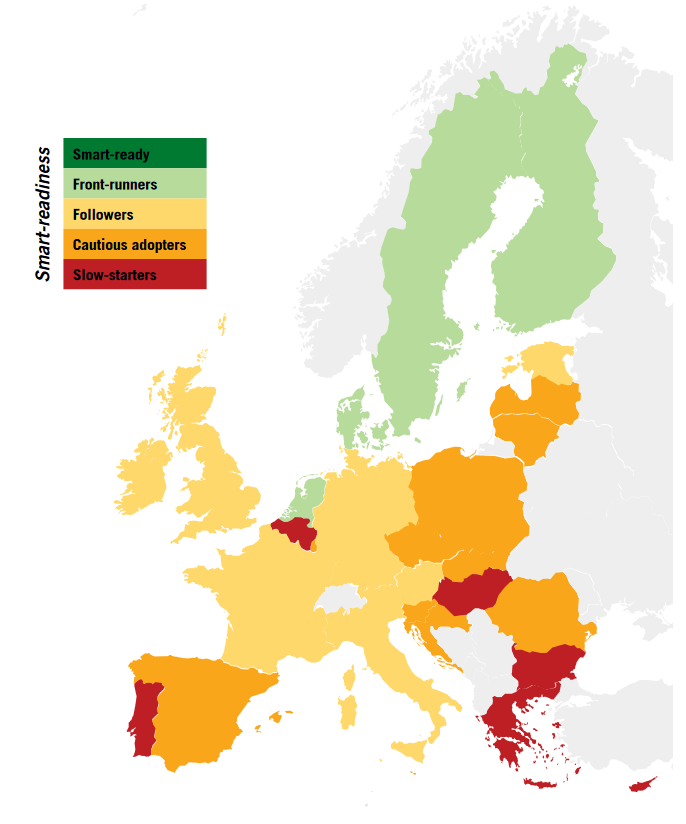
\includegraphics[width=\textwidth]{fig1}
\caption{A figure caption is always placed below the illustration.
Please note that short captions are centered, while long ones are
justified by the macro package automatically.} \label{fig1}
\end{figure}

For citations of references, we prefer the use of square brackets
and consecutive numbers. The following bibliography provides
a sample reference list with entries for journal
articles~\cite{ref_article1}, a book~\cite{ref_book1}, proceedings without editors~\cite{ref_proc1},
and a homepage~\cite{ref_url1}. Multiple citations are grouped
\cite{ref_article1,ref_book1},
\cite{ref_article1,ref_book1,ref_proc1,ref_url1}.

\section{System architecture}
Here goes the design of the system architecture.

\section{Requirements specification}
Here go the requirements both functional and non-functional of the system.

\section{Conclusions and Outlook}
Here goes the conclusions of the project and possible improvements as future work.

%
% ---- Bibliography ----
%
\bibliographystyle{splncs04}
\bibliography{mybib}

All links were last followed on April 17, 2019.

\end{document}
